\documentclass[11pt,a4paper]{report}

% ---------- fonts & encoding (match the reference report: Latin Modern via XeTeX) ----------
\usepackage[T1]{fontenc}
\usepackage{lmodern}

% ---------- core packages ----------
\usepackage{amsmath,amssymb}
\usepackage{graphicx}
\usepackage{xcolor}
\usepackage[a4paper,top=28mm,bottom=28mm,left=28mm,right=28mm,
            headheight=15pt,headsep=8mm,footskip=12mm]{geometry}
\usepackage{setspace}
\usepackage{booktabs}
\setlength{\tabcolsep}{5pt}
\usepackage{array}
\usepackage{tabularx}
\usepackage{caption}
\usepackage{enumitem}
\usepackage{fancyhdr}
\usepackage{needspace}
\usepackage{titlesec}
\titlespacing*{\chapter}{0pt}{18pt}{16pt}
\usepackage{tikz}
\usetikzlibrary{arrows.meta,positioning}
\usepackage[colorlinks=true,linkcolor=black,citecolor=black,urlcolor=blue,
            bookmarks=true,bookmarksnumbered=true]{hyperref}
\usepackage{microtype}

% ---------- layout ----------
\setstretch{1.08}
\setlength{\parskip}{1pt}
\tolerance=2000
\emergencystretch=1.5em
\widowpenalty=10000
\clubpenalty=10000
\setcounter{tocdepth}{0}
\setcounter{secnumdepth}{2}
\captionsetup{labelfont=bf,font=small,skip=5pt}
\setlist{itemsep=2pt,topsep=3pt,parsep=0pt}
\setlength{\textfloatsep}{13pt plus 2pt minus 4pt}
\setlength{\intextsep}{13pt plus 2pt minus 4pt}
\setlength{\floatsep}{11pt plus 2pt minus 3pt}

% ---------- headers & footers (same style as the reference report) ----------
\newcommand{\shorttitle}{Code-Mixed Hate Speech Detection in Hinglish: A Comparative Study of a TF-IDF Baseline and Three Multilingual Transformers}
\renewcommand{\chaptermark}[1]{\markboth{\MakeUppercase{\chaptername}\ \thechapter.\ \ #1}{}}
\renewcommand{\sectionmark}[1]{\markright{\MakeUppercase{\thesection}.\ \ #1}}
\pagestyle{fancy}
\fancyhf{}
\fancyhead[L]{\footnotesize\itshape\leftmark}
\fancyhead[R]{\footnotesize\itshape\rightmark}

\fancyfoot[L]{\footnotesize
  Hinglish Hate Speech Detection:\\
  TF-IDF vs. Multilingual Transformers}

\fancyfoot[C]{\thepage}
\fancyfoot[R]{\footnotesize VPKBIET, Baramati}
\renewcommand{\headrulewidth}{0.4pt}
\renewcommand{\footrulewidth}{0.4pt}
\fancypagestyle{plain}{%
  \fancyhf{}%
  \fancyfoot[C]{\thepage}%
  \renewcommand{\headrulewidth}{0pt}%
  \renewcommand{\footrulewidth}{0pt}%
}

% ---------- unnumbered chapter with TOC entry ----------
\newcommand{\frontchapter}[1]{%
  \chapter*{#1}\markboth{#1}{}\addcontentsline{toc}{chapter}{#1}}

% ---------- math shortcuts ----------
\newcommand{\mF}{F_{1}}
\newcommand{\mFmac}{F_{1}^{\mathrm{macro}}}

\renewcommand{\bibname}{References}

% ---------- PDF metadata ----------
\hypersetup{
  pdftitle={Mini Project Report on Code-Mixed Hate Speech Detection in Hinglish: A Comparative Study of a TF-IDF Baseline and Three Multilingual Transformers},
  pdfauthor={Anish Charudatta Date},
  pdfsubject={Deep Learning Mini Project Report, VPKBIET Baramati},
  pdfkeywords={Hate Speech Detection, Hinglish, Code-Mixed, TF-IDF, Transformer, RoBERTa, MuRIL, XLM-R, Macro-F1, McNemar}
}

\begin{document}

% =====================================================================
% TITLE PAGE
% =====================================================================
\begin{titlepage}
\centering
\includegraphics[width=34mm]{vpkbiet_logo.jpg}\par
\vspace{7mm}
{\large Mini Project Report on\par}
\vspace{4mm}
{\sffamily\bfseries\fontsize{19}{25}\selectfont
Hinglish Hate Speech Detection:\\
TF-IDF vs. Multilingual Transformers\par}
\vspace{12mm}
{\large Submitted in fulfillment of activity requirements\\
in the subject \textbf{Natural Language Processing}\par}
\vspace{7mm}
{\large BY\par}
\vspace{2mm}
{\large\bfseries Soham Nilesh Vaidya\par}
{\large\bfseries (Roll No.\ EN25552017)\par}
\vspace{2mm}
{\large\bfseries Anish Charudatta Date\par}
{\large\bfseries (Roll No.\ EN25552003)\par}
\vspace{7mm}
{\large Under the guidance of\par}
{\large Dr.\ A.\,M.\ Jagtap\par}
\par\vspace{10mm}
{\large Vidya Pratishthan's\\
Kamalnayan Bajaj Institute of Engineering and Technology\\
Baramati-413133, Dist-Pune (M.S.) India\\
Department of Computer Engineering\\[3mm]
November 2026-27\par}
\end{titlepage}

% =====================================================================
% CERTIFICATE
% =====================================================================
\pagenumbering{roman}
\thispagestyle{plain}
\noindent\rule{\textwidth}{0.4pt}\par
\vspace{5mm}
\begin{center}
\includegraphics[width=30mm]{vpkbiet_logo.jpg}\par
\vspace{2mm}
VPKBIET, Baramati\par
\vspace{5mm}
{\Huge\boldmath$\mathfrak{Certificate}$\par}
\vspace{7mm}
This is to certify that the Mini Project Report on\par
\vspace{3mm}
{\sffamily\bfseries\large
Code-Mixed Hate Speech Detection in Hinglish:\\
A Comparative Study of a TF-IDF Baseline and\\
Three Multilingual Transformers\par}
\vspace{4mm}
submitted by\par
\vspace{2mm}
{\bfseries Soham Nilesh Vaidya\par}
{\bfseries Roll No.\ EN25552017\par}
\vspace{4mm}
\begin{minipage}{0.88\textwidth}
in fulfillment of the activity requirements in the subject Natural Language Processing at Vidya
Pratishthan's Kamalnayan Bajaj Institute of Engineering and Technology, Baramati,
under the Savitribai Phule Pune University, Pune. This work is done during year
2026-27 Semester-III, under our guidance.
\end{minipage}\par
\end{center}
\vspace{16mm}
\noindent
\begin{tabular}{@{}p{0.42\textwidth}@{\hspace{0.04\textwidth}}p{0.23\textwidth}@{\hspace{0.04\textwidth}}p{0.23\textwidth}@{}}
 Dr.\ A.M.\ Jagtap & Dr.\ A.M.\ Jagtap & Dr.\ S.B.\ Lande\\[9mm]
Mini Project Guide & Head of Dept. & Principal\\
\end{tabular}
\vspace{16mm}

\noindent Examiner 1: \hrulefill \hfill Examiner 2: \hrulefill
\newpage

% =====================================================================
% FRONT MATTER
% =====================================================================
\pagenumbering{arabic}

\frontchapter{Acknowledgements}
I would like to express my sincere gratitude to my mini project guide,
Dr.\ A.\,M.\ Jagtap, who also heads the Department of Computer Engineering, for his
continuous guidance, patient review and constructive criticism throughout this
work. I am grateful to the Department of Computer Engineering for providing the
computational facilities that made the experiments possible. I also thank
Dr.\ S.\,B.\ Lande, Principal of VPKBIET, and all the faculty members of the
department, for their support and encouragement.

I thank the creators and maintainers of the PRISM Hinglish hate-speech dataset and
of the L3Cube-MeHate Marathi dataset, the L3Cube-Pune group and Google Research for
releasing the pretrained Hinglish and Indian-language models, and the Hugging Face,
\texttt{transformers} and scikit-learn communities, without whose open-source tools
this study could not have been carried out. I also thank Kaggle for providing the
GPU quota used for training. Finally, I thank my classmates for their comments
during the preparation of this report.

\frontchapter{Abstract}
\begingroup\footnotesize\setstretch{1.12}
Hate speech on Indian social media rarely arrives in pure English or pure Hindi:
it arrives as Hinglish---Hindi written in the Roman script, mixed with English in
the same sentence---and its non-standard spelling defeats word-level NLP tooling.
This report presents a controlled, reproducible comparison of four classifiers for
binary hate-speech detection on such code-mixed text: a lexical baseline built on
character $n$-gram TF-IDF features with a linear SVM (B0), and three fine-tuned
transformers spanning the pretraining spectrum---HingRoBERTa (romanised
Hindi--English), MuRIL (Indian languages) and XLM-RoBERTa (100-language generalist).
The experiments use the PRISM corpus (17{,}704 / 2{,}950 / 8{,}852 train,
validation and test posts, about 53.5\% non-hate) with the upstream revision pinned
and a data card written for every split. All four models share one protocol: three
seeds, macro-F1 as the single primary metric, the decision threshold tuned on the
validation set only, and the test set used exclusively for reporting; bootstrap
confidence intervals and Holm-corrected McNemar tests quantify uncertainty.

The result is a clear but modest gain for pretraining. The baseline reaches a test
macro-F1 of 0.7050; the three transformers reach 0.7300, 0.7254 and 0.7351
(HingRoBERTa, MuRIL and XLM-R respectively), so the best transformer buys about
three F1 points over the baseline while training roughly 96 times longer, and all
three gains are significant under McNemar with Holm correction (best
$p_{\mathrm{adj}} = 1.2\times10^{-13}$). The best backbone (XLM-R) is selected on the
validation set, so the reported test numbers carry no model-selection bias. The
error analysis locates the remaining weaknesses precisely: hate-class recall is the
lowest cell of the confusion matrix (0.645 for XLM-R), the code-mixed bucket of the
test set shows a 32.0\% error rate, and zero-shot transfer to Marathi--English
(L3Cube-MeHate) collapses macro-F1 from 0.7351 to 0.3770. The report closes with
a glossary appendix explaining every metric and term used.
\endgroup

{\let\clearpage\relax\chapter*{Keywords}\markboth{Keywords}{}\addcontentsline{toc}{chapter}{Keywords}}
\vspace{-2mm}
\noindent\textbf{Keywords---} Hate Speech Detection; Code-Mixed Language; Hinglish;
Text Classification; TF-IDF; Linear SVM; Transformer; HingRoBERTa; MuRIL; XLM-RoBERTa;
Fine-Tuning; Macro-F1; McNemar's Test; Bootstrap Confidence Interval; Zero-Shot Transfer.

\vspace{5mm}
\noindent\textbf{Abbreviations---} B0 (baseline model), A0 (advanced transformer
models), CI (confidence interval), EDA (exploratory data analysis), fp16
(16-bit floating point), GPU (graphics processing unit), HF (Hugging Face),
MCC (Matthews correlation coefficient), NLP (natural language processing),
PII (personally identifiable information), SVM (support vector machine),
TF-IDF (term frequency--inverse document frequency).

% =====================================================================
% CONTENTS
% =====================================================================
% CONTENTS
% =====================================================================
\begingroup
\footnotesize
\setstretch{1.0}
\setlength{\parskip}{0pt}

\setcounter{tocdepth}{1}
\tableofcontents

\clearpage
\listoftables

\listoffigures
\endgroup

% =====================================================================
% CHAPTERS
% =====================================================================
% =====================================================================
% CHAPTER 1 — INTRODUCTION
% =====================================================================
\chapter{Introduction}
\label{ch:intro}

\section{Research Background}
\label{sec:background}

Automatic moderation of abusive content is now a first-class requirement for
large social platforms, and its classical research formulation is hate-speech
detection: given a post, decide whether it contains hateful or attacking
language. On Indian platforms the task has a complication that most published
benchmarks barely address---the language itself. A large share of posts are
written in \emph{Hinglish}: Hindi expressed in the Roman script, freely mixed
with English inside the same sentence---\emph{``yeh kya bakwaas hai yaar''} in
one clause, English in the next, with no script boundary to mark the change.

This mixing is hostile to standard text pipelines in three concrete ways.
First, romanisation is non-phonetic: the same Hindi word appears as \emph{hai},
\emph{hain}, \emph{he} or \emph{hn}, so a word-level vocabulary fragments across
dozens of spelling variants. Second, word order and function words switch language
mid-sentence, so features built for one language generalise poorly to the other.
Third, abusive and identity terms are precisely the tokens most likely to be
romanised, abbreviated or obfuscated. Character-level features and pretrained
multilingual transformers are the two standard responses, at very different cost
points: a TF-IDF linear model trains in seconds, a fine-tuned transformer needs a
GPU and tens of minutes.

Pretrained models aimed at this language pair have recently appeared: HingRoBERTa
is an encoder further pretrained on romanised Hindi--English text
\cite{hingroberta,nayak2022}, MuRIL covers Indian languages including Devanagari
Hindi \cite{muril}, and XLM-RoBERTa covers one hundred languages \cite{xlmr}.
What they promise is what the lexical baseline lacks---subword robustness and
prior knowledge. Whether that promise converts into measurable accuracy on a
public Hinglish benchmark, under a fixed and honest evaluation protocol, is the
subject of this report.

\section{Problem Statement}
\label{sec:problem}

The core question of this study is: \emph{on a public Hinglish hate-speech
benchmark, and under an identical training and evaluation protocol, how much
accuracy does pretrained multilingual pretraining buy over a character-level
lexical baseline---and where exactly does the additional cost still fail?}

Three sub-questions make this concrete. First, does fine-tuning a transformer
beat the TF-IDF + linear-SVM baseline by a margin that survives multiple seeds and
a statistical significance test, or is the gain within seed noise? Second, does
the \emph{domain} of pretraining matter---romanised Hinglish (HingRoBERTa),
Devanagari Indian languages (MuRIL), or a broad multilingual generalist
(XLM-R)---for a task whose test text is mostly Roman script? Third, on which
segments of the data do the models still fail: the hate class, the code-mixed
posts, or text outside the training language, measured by a zero-shot transfer
test to Marathi--English?

A fourth concern is methodological rather than empirical: the numbers must be
trustworthy. In an earlier version of this pipeline (v1), the transformer backbone
was selected on \emph{test} macro-F1, which leaks test information into the
model-selection decision and biases every reported test score. Version 2, reported
here, enforces a strict discipline---all decisions (threshold, checkpoint, backbone)
are made on the validation set, and the test set is touched once, for reporting.
The protocol itself is therefore part of the contribution.

\begin{figure}[htbp]
\centering
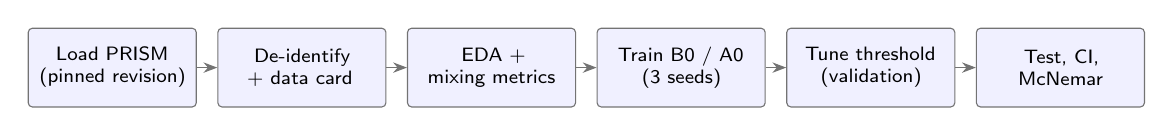
\begin{tikzpicture}[
  node distance=2.6mm,
  box/.style={draw=black!55, rounded corners=1.5pt, fill=blue!6,
              minimum height=10mm, text width=19mm, align=center,
              font=\scriptsize\sffamily},
  arr/.style={-{Stealth[length=5pt]}, black!55}]
  \node[box] (a) {Load PRISM\\(pinned revision)};
  \node[box, right=of a] (b) {De-identify\\+ data card};
  \node[box, right=of b] (c) {EDA +\\mixing metrics};
  \node[box, right=of c] (d) {Train B0 / A0\\(3 seeds)};
  \node[box, right=of d] (e) {Tune threshold\\(validation)};
  \node[box, right=of e] (f) {Test, CI,\\McNemar};
  \draw[arr] (a) -- (b);
  \draw[arr] (b) -- (c);
  \draw[arr] (c) -- (d);
  \draw[arr] (d) -- (e);
  \draw[arr] (e) -- (f);
\end{tikzpicture}
\caption[The experimental pipeline shared by all four models]{The experimental pipeline shared by all four models. Every stage writes
checksummed artifacts; the test labels are used only in the final stage.}
\label{fig:pipeline}
\end{figure}

\section{Scope of the Study}
\label{sec:scope}

Within the scope of this study are: binary (hate / non-hate) classification;
the PRISM Hindi--English corpus as the only training resource \cite{prism}; three
seeds per model; one fixed hyperparameter set shared by all transformers; and a
single zero-shot transfer evaluation to L3Cube-MeHate \cite{mehate} without any
training on it.

Outside the scope are: multiclass or target-group labelling (PRISM provides binary
labels only); training on Marathi or any other transfer language; domain
adaptation, ensembling and model compression; large-scale hyperparameter search;
and deployment or latency optimisation. Where the data forces a limitation---for
example, the MeHate transfer set is the small 416-row code-mixed test split---the
limitation is stated explicitly in the text rather than silently absorbed.

\section{Main Contributions}
\label{sec:contrib}

The work of this report can be summarised in five points.

\begin{itemize}
\item \textbf{A leakage-safe evaluation protocol, fixed in code.} The decision
threshold is tuned on the validation set only, the checkpoint and the best backbone
are selected on validation macro-F1, and the test set is scored once per seed.
Version 2 of the pipeline repairs a concrete v1 defect where the backbone was
chosen on test macro-F1 (\S\ref{sec:protocol}).
\item \textbf{A controlled four-model comparison.} One baseline and three
transformers are trained under an exactly identical recipe---same splits, same
metric, same seeds---so the comparison isolates the effect of pretraining rather
than of protocol differences.
\item \textbf{A code-mixing metric that can actually see Romanised Hinglish.}
Version 1 measured the Devanagari script ratio, which assigns Romanised Hinglish a
mixing score of zero. Version 2 performs word-level language identification using
a compact romanised-Hindi lexicon, yielding a mixing index and word-level
code-switch counts (\S\ref{sec:mixing}).
\item \textbf{Statistical grounding.} Every headline number is a 3-seed mean with
a bootstrap confidence interval around the mean, and every baseline-vs-transformer
claim is backed by an exact McNemar test with Holm correction
(\S\ref{sec:stats}).
\item \textbf{A failure map, not only a leaderboard.} Performance is decomposed by
language and by mixing bucket, and probed out of domain by a zero-shot transfer
test, so the report states \emph{where} the three extra F1 points do not reach
(\S\ref{sec:errors}--\S\ref{sec:transfer}).
\end{itemize}

\section{Organisation of the Report}
\label{sec:org}

Chapter~\ref{ch:method} details the datasets, the de-identification rules, the
exploratory analysis, the four models, the training protocol and the evaluation
methodology. Chapter~\ref{ch:results} presents the results: the main comparison,
statistical significance, cost, training behaviour, error analysis and the
cross-lingual transfer test. Chapter~\ref{ch:conclusion} states the conclusions, the limitations and the future
work. Appendix~A provides a glossary of all technical terms and evaluation metrics
used in the report, written so that a reader new to NLP evaluation can follow every
table.

% =====================================================================
% CHAPTER 2 — METHODOLOGY
% =====================================================================
\chapter{Methodology}
\label{ch:method}

\section{Datasets}
\label{sec:data}

\subsection{PRISM: the primary Hinglish corpus}
The experiments use the PRISM Hinglish hate-speech dataset \cite{prism}, a
publicly available corpus of social-media posts labelled for hate speech, with
posts in English, Hindi (Devanagari) and Hinglish (Roman script). The upstream
repository revision is pinned by SHA (\texttt{b27f83eb\ldots}), the row counts are
asserted against the dataset card at load time, and each processed split is
written to disk with a SHA-256 checksum so that the exact data behind every
number cannot drift silently.

Table~\ref{tab:prism} reports the three official splits. The corpus is close to
balanced---about 53.5\% non-hate and 46.5\% hate in every split---so accuracy
alone is not misleading here, but macro-averaged metrics are still the safer
primary choice, and they are used throughout. The language distribution is the
more consequential property: by design, a substantial fraction of the corpus is
Roman-script Hinglish, which is the segment that standard tooling handles worst.

\begin{table}[htbp]
\centering
\caption[PRISM splits and label balance]{PRISM splits and label balance (verified against the pinned revision).}
\label{tab:prism}
\small
\begin{tabular}{lrrrr}
\toprule
Split & Posts & Non-hate (\%) & Hate (\%) & Purpose \\
\midrule
Train & 17{,}704 & 53.5 & 46.5 & Model fitting \\
Validation & 2{,}950 & 53.6 & 46.4 & All decisions \\
Test & 8{,}852 & 53.5 & 46.5 & Reporting only \\
\midrule
Total & 29{,}506 & 53.5 & 46.5 & \\
\bottomrule
\end{tabular}
\end{table}

Class share also varies by language. In the training split, English posts are
exactly balanced (50.0\% / 50.0\%), Hindi posts lean non-hate (55.2\% / 44.8\%),
and Hinglish posts lean non-hate most strongly (61.2\% / 38.8\%). Any
per-language comparison in Chapter~\ref{ch:results} must be read against these
different base rates.

\subsection{L3Cube-MeHate: the transfer set}
For the cross-lingual probe we use L3Cube-MeHate \cite{mehate}, a Marathi and
Marathi--English code-mixed hate-speech corpus. Only its small code-mixed
\emph{test} split is used---416 posts, 50\% / 50\% balanced---and only in zero-shot
mode: no training, no validation, no threshold re-tuning. The GitHub commit is
pinned (\texttt{8ee29fa\ldots}) and the sentiment and profanity columns shipped
with the file are deliberately ignored, keeping the label space identical to
PRISM's. Both the small split size and the single-test-split usage are stated
here as disclosed limitations rather than hidden choices.

\section{De-identification}
\label{sec:deid}

Social-media text carries personally identifiable information, and a hate-speech
corpus is exactly where it concentrates. Before any analysis, five
regular-expression rules are applied to every post of every split
(Table~\ref{tab:deid}). The rules are deliberately conservative: emojis are kept
(they are signal in this task), digit runs survive unless they look like phone
numbers, and letter elongation is collapsed for alphabetic characters only
(\emph{sooooo} $\rightarrow$ \emph{soo}).

\begin{table}[htbp]
\centering
\caption{De-identification rules applied to all splits.}
\label{tab:deid}
\small
\begin{tabular}{llp{6.2cm}}
\toprule
Pattern & Replacement & Notes \\
\midrule
URL / \texttt{www.} & \texttt{<URL>} & http(s) and bare domains \\
Email address & \texttt{<EMAIL>} & standard address pattern \\
Phone number & \texttt{<PHONE>} & $\geq$8 digits incl.\ separators \\
\texttt{@handle} & \texttt{<USER>} & mentions removed \\
Letter elongation & doubled letter & alphabetic runs only \\
\bottomrule
\end{tabular}
\end{table}

One caveat must be stated: the de-identification is regex-based, so full names
written in plain text are \emph{not} removed. This is recorded in the data card
written next to the processed splits, and it is why the processed CSVs are treated
as sensitive artifacts rather than publishable data.

\section{Exploratory Analysis and the Code-Mixing Metric}
\label{sec:eda}

\subsection{Class balance and text length}
Class share varies by language (Figure~\ref{fig:classbalance}): in the training
split, English posts are exactly balanced (50.0\% / 50.0\%), Hindi posts lean
non-hate (55.2\% / 44.8\%), and Hinglish posts lean non-hate most strongly
(61.2\% / 38.8\%). Length adds a second asymmetry: non-hate posts are longer on
average (mean 32.4 words, median 19, maximum 300) than hate posts (mean 23.7,
median 16, maximum 295), consistent with the short, direct register of abusive
attacks. Both properties matter later: any per-language comparison in
Chapter~\ref{ch:results} must be read against these different base rates, and
length is a weak but real cue that must not be confused with language effects.

\begin{figure}[htbp]
\centering
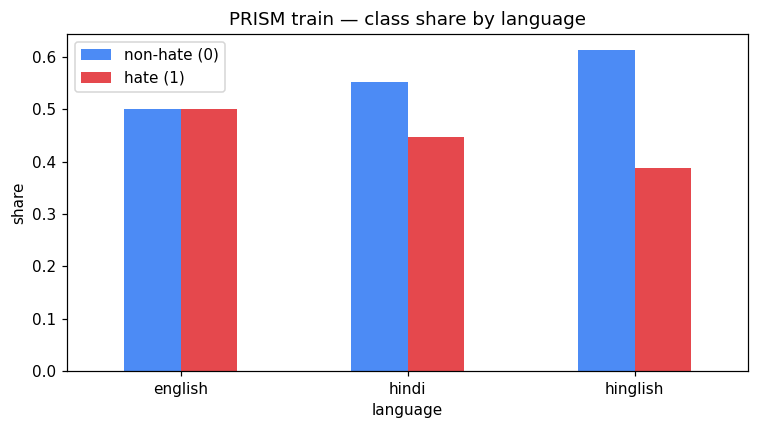
\includegraphics[width=0.62\textwidth]{figures/fig_class_balance.png}
\caption{PRISM training split---class share by language. Hinglish posts lean
non-hate (61.2\% / 38.8\%) while English posts are exactly balanced.}
\label{fig:classbalance}
\end{figure}

\subsection{Measuring code-mixing at the word level}
\label{sec:mixing}
Quantifying ``how mixed is this post'' is a prerequisite for the error analysis in
Chapter~\ref{ch:results}, and the obvious script-based measure is blind here: v1
of the pipeline measured the Devanagari character ratio, which by definition
assigns Romanised Hinglish a mixing score of exactly zero. Version 2 therefore
classifies each word token as Hindi or English: Devanagari tokens count as Hindi,
tokens in a compact romanised-Hindi lexicon (function words, common adverbs, and
frequent content terms including profanity, with common transliteration variants)
count as Hindi, and the remaining Latin tokens count as English. Placeholder
tokens and punctuation are excluded so that they cannot create phantom switches.

From these token labels the pipeline computes four statistics per post:
the Hindi token ratio; the \emph{mixing index}, defined as the minority-language
token share $\mathrm{MI} = \min(n_{\mathrm{hi}}, n_{\mathrm{en}})/n$ (0 for
monolingual text, 0.5 for a balanced mix); the number of adjacent word-level
code-switch points; and the Devanagari character ratio, kept as a script
covariate. The lexicon approach has a stated bias: content words absent from the
lexicon are counted as English, so the mixing index is a \emph{lower bound} on
true mixing.

The measurements confirm the metric can see the phenomenon
(Table~\ref{tab:mixing}). Romanised Hinglish posts average a mixing index of 0.307
with 8.5 word-level switch points per post, while pure-English posts average 0.062
(their Hindi share comes from unambiguous romanised tokens such as \emph{yaar}) and
pure-Hindi posts are exactly monolingual. Mixing is also mildly class-linked:
within Hinglish, non-hate posts mix slightly more (0.325) than hate posts (0.279),
and Figure~\ref{fig:codemixing} shows the full distributions.

\begin{table}[htbp]
\centering
\caption[Code-mixing statistics by language]{Code-mixing statistics by language (training split, means per post).}
\label{tab:mixing}
\small
\begin{tabular}{lrrr}
\toprule
Language & Hindi token ratio & Mixing index & Switch points \\
\midrule
English & 0.062 & 0.062 & 5.07 \\
Hindi & 1.000 & 0.000 & 0.00 \\
Hinglish & 0.323 & 0.307 & 8.47 \\
\bottomrule
\end{tabular}
\end{table}

\begin{figure}[htbp]
\centering
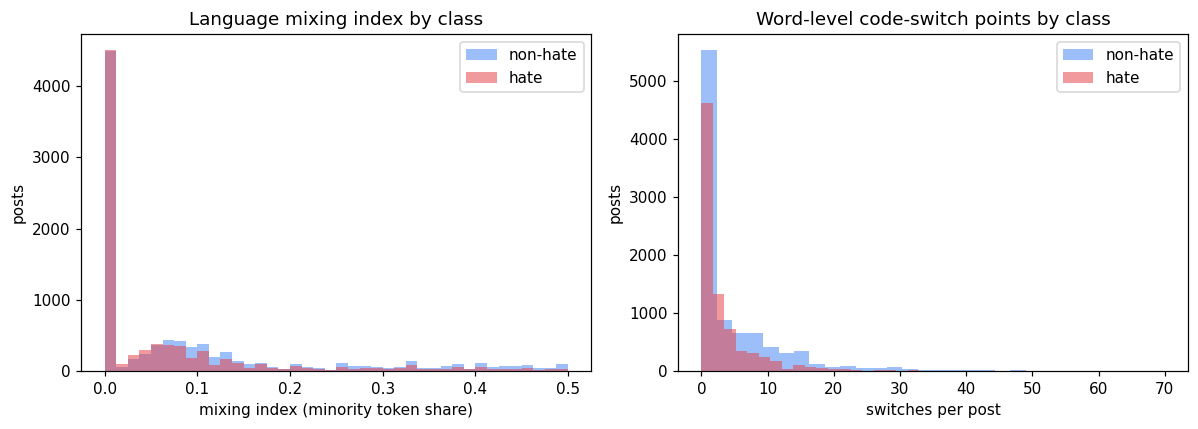
\includegraphics[width=0.8\textwidth]{figures/fig_code_mixing.png}
\caption{Language-mixing index (left) and word-level code-switch points (right)
by class. Romanised Hinglish is now visible to the metric; in v1 it scored zero.}
\label{fig:codemixing}
\end{figure}

\section{Models}
\label{sec:models}

Four classifiers are compared under one protocol. They are deliberately chosen to
span the design space from ``no learning beyond counting'' to ``pretraining on
exactly this language mixture''.

\subsection{B0 --- character $n$-gram TF-IDF + linear SVM}
The baseline vectorises each post with character $n$-grams ($n = 2$ to 5),
lowercased, minimum document frequency 2, at most 300{,}000 features with
sublinear TF weighting, and classifies with a linear support vector machine
($C = 1.0$) \cite{sklearn}. Character features are the classical answer to
romanisation noise---\emph{hain}, \emph{he} and \emph{hn} match through shared
substrings instead of exact word identity---and the model trains on CPU in
seconds. It is deterministic given the seed; its three seed runs produce
identical predictions.

\subsection{A0 --- three fine-tuned transformers}
The three transformer classifiers share the \texttt{AutoModelForSequenceClassification}
harness with a freshly initialised binary classification head, differing only in
the pretrained checkpoint that is loaded
(Table~\ref{tab:models}). The trio tests the ``does pretraining domain matter''
question: HingRoBERTa was further pretrained on $\sim$1B tokens of romanised
Hindi--English text and is the domain-matched candidate \cite{hingroberta,nayak2022};
MuRIL was pretrained on Indian-language corpora including Devanagari Hindi and is
the script-matched candidate \cite{muril}; XLM-RoBERTa is the 100-language
generalist with no special exposure to Hinglish \cite{xlmr}. All heads are trained
from scratch on PRISM; only the encoder weights come from pretraining.

\begin{table}[htbp]
\centering
\caption[The four models and their parameter counts]{The four models. ``Params'' is the fine-tuned parameter count.}
\label{tab:models}
\small
\begin{tabular}{p{2.6cm}p{4.6cm}rp{3.4cm}}
\toprule
Model & Checkpoint & Params & Rationale \\
\midrule
B0 & TF-IDF char 2--5 grams + LinearSVC & --- & Lexical control; CPU; noise-robust \\
HingRoBERTa & \texttt{l3cube-pune/hing-roberta} & 278.0\,M & Pretrained on romanised Hinglish \\
MuRIL & \texttt{google/muril-base-cased} & 237.6\,M & Indian languages, Devanagari-strong \\
XLM-RoBERTa & \texttt{xlm-roberta-base} & 278.0\,M & 100-language generalist \\
\bottomrule
\end{tabular}
\end{table}

\section{Training Protocol}
\label{sec:training}

All transformer runs use one training loop and one hyperparameter set
(Table~\ref{tab:hyperparams}), so no model can win by configuration shopping. The
checkpoint restored at the end of training is the one with the best
\emph{validation} macro-F1, not the last epoch, and fp16 mixed precision is
enabled on GPU.

\begin{table}[htbp]
\centering
\caption[Training configuration shared by all transformer runs]{Training configuration shared by all transformer runs (full-run mode).}
\label{tab:hyperparams}
\small
\begin{tabular}{ll}
\toprule
Setting & Value \\
\midrule
Maximum sequence length & 128 subword tokens \\
Epochs & 3 \\
Batch size (train / eval) & 32 / 64 \\
Learning rate & $2\times10^{-5}$ (AdamW) \\
Weight decay / warmup ratio & 0.01 / 0.1 \\
Precision & fp16 on GPU \\
Seeds & 42, 43, 44 (seeded in torch and HF) \\
Checkpoint selection & Best validation macro-F1 \\
Logging / reporting & every 50 steps / none (files only) \\
\bottomrule
\end{tabular}
\end{table}

Three implementation choices deserve note because they protect the results rather
than decorate them. First, the three seeds are genuine repetitions: seed 42's
artifacts are kept resident for the error analysis, while seeds 43 and 44 are
trained, scored, and explicitly deleted from GPU memory before the next run.
Second, predictions of every run are saved as arrays before any metric is
computed, so the significance tests later reuse exactly the training-time outputs.
Third, a smoke-test mode (tiny model, four optimiser steps, CPU-allowed) lets the
full pipeline be exercised end-to-end in about two minutes before spending GPU
hours; a fail-fast assertion refuses the full run when no GPU is present, because
a CPU run would silently drop fp16 and change the experiment.

\section{Evaluation Protocol and Metrics}
\label{sec:protocol}

\subsection{Metrics}
Five dataset-level metrics are computed for every run: macro precision, macro
recall, macro-F1, the Matthews correlation coefficient (MCC) and balanced
accuracy. \emph{Macro-F1} is the single primary metric: it averages the F-scores
of the two classes equally, so a model cannot hide a collapsing minority class
behind the majority one. MCC and balanced accuracy are robustness checks---MCC
summarises the whole confusion matrix, balanced accuracy exposes recall imbalance.
Per-class scores are analysed in \S\ref{sec:perclass}; formal definitions of
every metric are collected in Appendix~A.

\subsection{The decision threshold is a tuned parameter}
The transformers output class probabilities, and the default rule ``predict hate
if $p \geq 0.5$'' is itself a modelling choice. The pipeline therefore sweeps the
threshold from 0.05 to 0.95 in steps of 0.01, evaluates macro-F1 at each value
\emph{on the validation set only}, and carries the argmax threshold to the test
set. Chosen thresholds ranged from 0.46 to 0.53 across the nine runs---a range
that brackets 0.5 without being centred on it; Section~\ref{sec:threshold}
quantifies how much the tuning matters. The baseline is unaffected: a linear SVM
has no probability output, so its boundary is fixed.

\subsection{Which numbers may be used for which decision}
The protocol distinguishes three information channels, and the distinction is the
central methodological fix of v2:
\begin{itemize}
\item \textbf{Validation macro-F1} drives every decision: per-epoch checkpoint
selection, threshold tuning, and the choice of the best A0 backbone for the
error analysis and the transfer test.
\item \textbf{Test macro-F1} (3-seed mean $\pm$ standard deviation, plus a
bootstrap 95\% CI around the mean, 1{,}000 resamples \cite{bootstrap}) is for
reporting only.
\item \textbf{Significance testing} (exact McNemar \cite{mcnemar} on the seed-42
test predictions, Holm-corrected across the three comparisons \cite{holm})
answers whether each transformer beats B0, not which transformer is best.
\end{itemize}
In v1, the backbone for the error analysis was chosen on \emph{test} macro-F1; the
v1-vs-v2 ranking of the backbones differs, which is exactly the bias this fix
removes. All reported v2 numbers use the validation-selected backbone
(XLM-R, mean validation macro-F1 0.7488 vs.\ 0.7423 and 0.7363).

\section{Statistical Testing}
\label{sec:stats}

Two complementary procedures quantify uncertainty. \emph{Bootstrap confidence
intervals}: the test set is resampled with replacement 1{,}000 times; within each
resample, macro-F1 is computed for each of the three seeds and averaged, so the
interval is centred on the plotted 3-seed mean rather than on one lucky seed.
\emph{McNemar's test}: for each transformer vs.\ the baseline, the exact binomial
test is applied to the discordant pairs---the test items where exactly one of the
two models is correct---which is the appropriate test for paired predictions on a
fixed test set. Because three transformers are compared against the same baseline,
the three $p$-values are Holm-corrected; the correction is performed and reported
explicitly rather than left to the reader.

\section{Implementation Environment}
\label{sec:environment}

The full run executes in a single Kaggle notebook on an NVIDIA T4 GPU (fp16
enabled), using \texttt{transformers} $\geq$ 4.46 (for \texttt{eval\_strategy}
and \texttt{processing\_class} semantics), \texttt{datasets} $\geq$ 3.0,
\texttt{accelerate}, scikit-learn and SciPy \cite{transformers,sklearn}. Every
stage writes to one results tree (\texttt{results/}, \texttt{figures/},
\texttt{preds/}) with a \texttt{run\_manifest.json} and a
\texttt{requirements-freeze.txt} snapshot, so each number in
Chapter~\ref{ch:results} traces to a file.

% =====================================================================
% CHAPTER 3 — RESULTS AND DISCUSSION
% =====================================================================
\chapter{Results and Discussion}
\label{ch:results}

\section{Baseline Results}
\label{sec:baseline}

The B0 baseline is strong for its cost: validation macro-F1 0.7093, test
macro-F1 0.7050 (MCC 0.4104, balanced accuracy 0.7047, bootstrap 95\% CI
$[0.6957, 0.7144]$). Training one seed takes 8.9 seconds and inference 0.50\,ms
per post. Its three seed runs are bit-identical (std $= 0.0000$), as expected for
a deterministic linear model---all seed variance in this study belongs to the
transformers, and the CI of the mean is correspondingly narrow. Two practical
readings follow: 0.7050 macro-F1 from a CPU model is a real bar that any
transformer must justify a GPU to beat, and the McNemar comparisons of
\S\ref{sec:significance} have a clean, noise-free reference.

\section{Main Comparison on the Test Set}
\label{sec:main}

Table~\ref{tab:main} reports the primary result: test macro-F1 as the 3-seed mean
$\pm$ standard deviation, the bootstrap 95\% CI around that mean, and the two
robustness metrics. Figure~\ref{fig:mainci} visualises the means with their CIs.

\begin{table}[htbp]
\centering
\caption[Main results on the PRISM test set]{Main results on the PRISM test set (3-seed mean $\pm$ std; CI is a
bootstrap 95\% interval around the mean, 1{,}000 resamples).}
\label{tab:main}
\small
\begin{tabular}{lrrrrr}
\toprule
Model & Macro-F1 & 95\% CI & MCC & Bal.\ acc. & Threshold \\
\midrule
B0 TF-IDF + SVM & 0.7050 $\pm$ 0.0000 & [0.6957, 0.7144] & 0.4104 & 0.7047 & --- \\
HingRoBERTa & 0.7300 $\pm$ 0.0046 & [0.7214, 0.7386] & 0.4639 & 0.7292 & 0.48 \\
MuRIL & 0.7254 $\pm$ 0.0036 & [0.7168, 0.7343] & 0.4582 & 0.7245 & 0.51 \\
XLM-RoBERTa & \textbf{0.7351 $\pm$ 0.0064} & [0.7265, 0.7439] & \textbf{0.4794} & \textbf{0.7344} & 0.51 \\
\bottomrule
\end{tabular}
\end{table}

\begin{figure}[htbp]
\centering
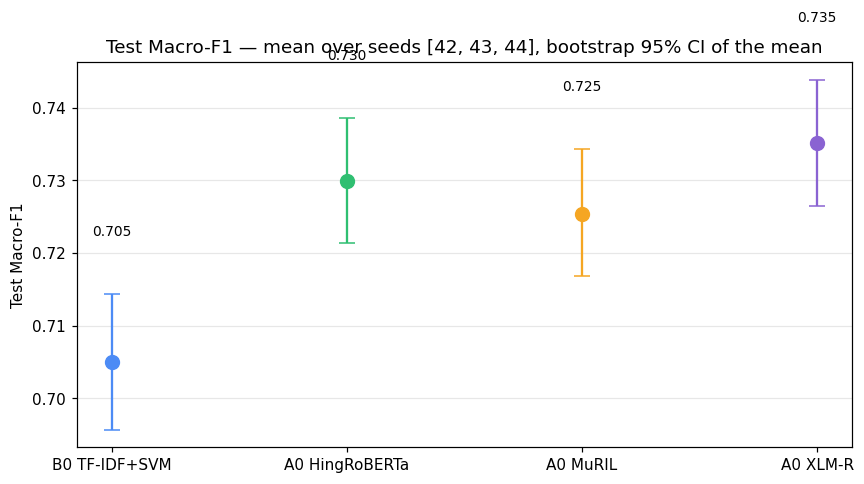
\includegraphics[width=0.66\textwidth]{figures/fig1_macro_f1_ci.png}
\caption[Test macro-F1: 3-seed mean with bootstrap 95\% CI]{Test macro-F1: 3-seed mean with bootstrap 95\% CI of the mean. The
transformer CIs sit above the baseline's, and largely above it outright.}
\label{fig:mainci}
\end{figure}

Three observations. First, \emph{pretraining wins, but modestly}: the best
transformer (XLM-R, 0.7351) beats the baseline by 0.0301 macro-F1, and the gap
between the best and worst transformer (0.0097) is smaller than the gap between
any transformer and the baseline. Second, \emph{the domain-matched model is not
the winner}: HingRoBERTa scores 0.7300, below the generalist XLM-R, though their
confidence intervals overlap heavily---the honest reading is ``XLM-R and
HingRoBERTa are statistically close; MuRIL trails both''. Third, \emph{seed noise
is real but small}: transformer stds (0.0036--0.0064) are an order of magnitude
below the baseline gap, so the ranking is not a one-seed accident---and
\S\ref{sec:significance} makes this precise.

\section{Per-Class Behaviour}
\label{sec:perclass}

Figure~\ref{fig:perclass} decomposes the headline numbers. The pattern is uniform
across all four models: the \emph{hate} class is the hard one. For XLM-R, hate
precision is actually the best in the table (0.762), but hate recall is the worst
cell (0.645)---the model misses roughly one hate post in three. Non-hate recall
for the transformers (0.79--0.82) exceeds hate recall by 13--18 points. The
baseline shows the same asymmetry in weaker form (hate recall 0.670).

Two consequences follow. First, the models are conservative: they prefer to label
an ambiguous post non-hate, which in a moderation pipeline means human review
queues absorb the misses. Second, because \emph{every} model shares this shape,
the cause is more likely in the data than in the architecture---boundary cases
where hateful intent is implied without explicit profanity are exactly the posts
that romanised, code-mixed text makes hardest to verify. This motivates the
threshold analysis in \S\ref{sec:threshold}: shifting the operating point trades
precision for recall directly.

\begin{figure}[htbp]
\centering
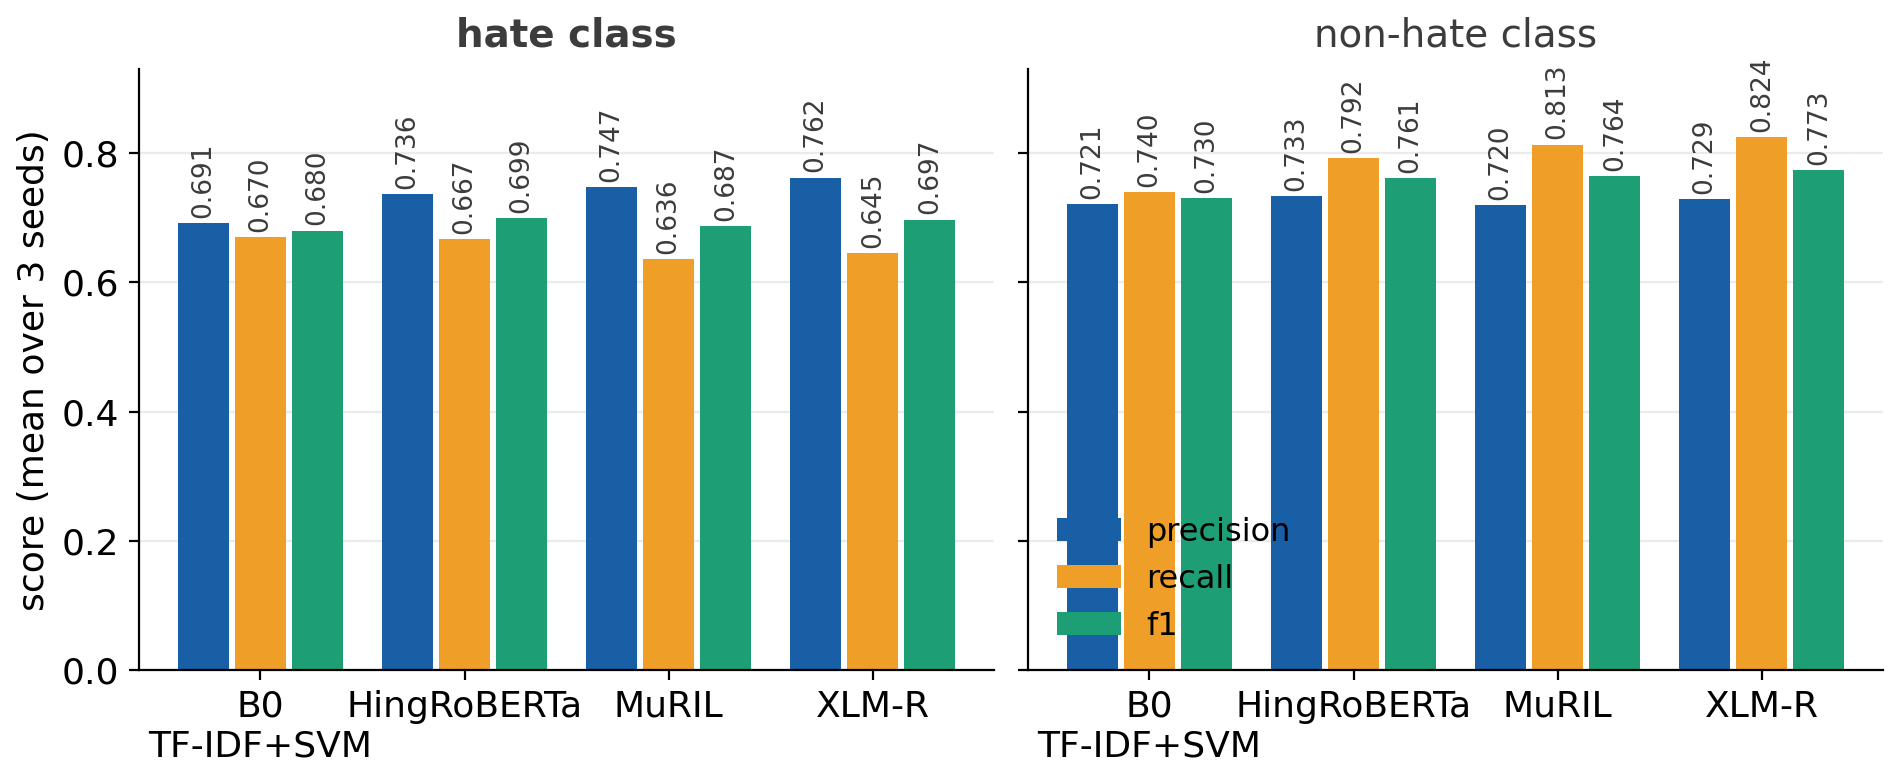
\includegraphics[width=0.98\textwidth]{figures/fig_per_class.png}
\caption[Per-class precision / recall / F1 on the test set]{Per-class precision / recall / F1 on the test set (mean over seeds).
Hate recall is the weakest cell for every model.}
\label{fig:perclass}
\end{figure}

\section{Statistical Significance}
\label{sec:significance}

Table~\ref{tab:mcnemar} reports the exact McNemar tests of each transformer
against B0 on the seed-42 test predictions, with Holm-corrected $p$-values across
the three comparisons. Every transformer wins: the discordant counts favour the
transformer in all three cases, and even the smallest margin (MuRIL: 1{,}094 vs.\
919 posts) is decisive after correction ($p_{\mathrm{adj}} = 3.1\times10^{-4}$).

\begin{table}[htbp]
\centering
\caption[Exact McNemar tests vs.\ B0 with Holm correction]{Exact McNemar tests vs.\ B0 (seed 42, $n = 8{,}852$). $n_{01}$: B0
correct, transformer wrong; $n_{10}$: transformer correct, B0 wrong. Holm
correction over the three comparisons.}
\label{tab:mcnemar}
\small
\begin{tabular}{lrrrl}
\toprule
Comparison & $n_{10}$ & $n_{01}$ & $p$ (exact) & $p$ (Holm-adj.) \\
\midrule
HingRoBERTa $>$ B0 & 1{,}263 & 980 & $2.5\times10^{-9}$ & $7.5\times10^{-9}$ \\
MuRIL $>$ B0 & 1{,}094 & 919 & $1.0\times10^{-4}$ & $3.1\times10^{-4}$ \\
XLM-R $>$ B0 & 1{,}181 & 841 & $4.1\times10^{-14}$ & $1.2\times10^{-13}$ \\
\bottomrule
\end{tabular}
\end{table}

Note what the test does and does not claim. It establishes that each transformer
is \emph{better than the baseline} on this test set, not that XLM-R is better than
HingRoBERTa---comparisons among the transformers were not tested, and given the
overlapping CIs of Table~\ref{tab:main} they would need more seeds to be
meaningful. The Holm correction is what licenses the word ``significant'' at all:
three uncorrected tests at $\alpha = 0.05$ would inflate the family-wise error
rate to about 14\%.

\section{Cost versus Quality}
\label{sec:cost}

Table~\ref{tab:costs} puts the accuracy table next to its price tag. Training a transformer seed takes 823--857 seconds against the
baseline's 8.9---a factor of about $96\times$ for XLM-R---and inference runs at
6.6\,ms per post against 0.50\,ms, a $13\times$ slowdown. The bought commodity is
$+0.0301$ macro-F1.

\begin{table}[htbp]
\centering
\caption[Cost of each model (mean over seeds)]{Cost of each model (mean over seeds). Training time excludes tokenisation
and data loading; inference is measured over the full test set.}
\label{tab:costs}
\small
\begin{tabular}{lrrr}
\toprule
Model & Params & Train time/seed & Inference \\
\midrule
B0 TF-IDF + SVM & --- & 8.9\,s & 0.50\,ms/post \\
HingRoBERTa & 278.0\,M & 856\,s & 6.56\,ms/post \\
MuRIL & 237.6\,M & 823\,s & 6.88\,ms/post \\
XLM-RoBERTa & 278.0\,M & 857\,s & 6.60\,ms/post \\
\bottomrule
\end{tabular}
\end{table}

Whether $96\times$ training and $13\times$ inference for three F1 points is a
good trade depends on the deployment. For a queue that screens millions of posts
the inference ratio alone is decisive: at 6.6\,ms per post one GPU core handles
$\sim$150 posts/s, the SVM $\sim$2{,}000 on CPU. A defensible hybrid reading is
to use the transformer where its three points matter most---the ambiguous middle
of the score distribution---and the SVM for the obvious remainder; this study
does not build that cascade, and lists it as future work (\S\ref{sec:future}).

\section{Training Behaviour and the Decision Threshold}
\label{sec:threshold}

The training dynamics are consistent across the transformers: training loss falls
steeply in the first epoch and validation macro-F1 rises with it, with most of the
achievable gain already present after the first of the three epochs. This explains
why the fixed three-epoch budget is not obviously under-provisioned for
fine-tuning, and it shows the plateau that the checkpoint policy (best validation
macro-F1) is designed to catch.

The validation macro-F1 surface over the swept threshold is flat near each
transformer's optimum---macro-F1 varies by less than half a point over a
$\pm$0.05 window---so the exact threshold is not a sensitive parameter. Table~\ref{tab:thresholds} makes the same point from the
other side: on the test set, the tuned threshold buys at most $+0.0022$ macro-F1
over the default argmax rule for XLM-R, and for MuRIL the tuned value is
marginally \emph{lower} than argmax. The value of the sweep is not the points it
buys but the bias it avoids: it removes ``0.5 was used by default'' as an
unexamined choice, and it moves one decision out of the test set.

\begin{table}[htbp]
\centering
\caption[Validation-tuned threshold vs.\ fixed 0.5 (seed 42)]{Validation-tuned threshold vs.\ fixed 0.5 (argmax) on the test set,
seed 42.}
\label{tab:thresholds}
\small
\begin{tabular}{lrrr}
\toprule
Model & Tuned thr. & Test F1 (tuned) & Test F1 (argmax) \\
\midrule
HingRoBERTa & 0.47 & 0.7363 & 0.7341 \\
MuRIL & 0.51 & 0.7206 & 0.7211 \\
XLM-RoBERTa & 0.53 & 0.7424 & 0.7408 \\
\bottomrule
\end{tabular}
\end{table}

\section{Error Analysis}
\label{sec:errors}

The error analysis uses the validation-selected backbone (XLM-R, seed 42) and
compares it to B0 throughout.

\subsection{Where the errors live: language and mixing level}
\label{sec:errors:lang}
Table~\ref{tab:perlang} splits the test set by post language. English posts are
the easiest for both models, and the transformer's advantage concentrates there
($+0.047$ macro-F1 over B0). Hindi and Hinglish posts are markedly harder; on
Hindi, the transformer's gain is nearly zero ($+0.002$). Since the test set
contains 2{,}900 Hindi and 1{,}407 Hinglish posts, a full third of the data
contributes almost none of the improvement.

\begin{table}[htbp]
\centering
\caption[Test macro-F1 by post language]{Test macro-F1 by post language (seed 42, $n$ = posts).}
\label{tab:perlang}
\small
\begin{tabular}{lrrr}
\toprule
Language & $n$ & B0 & A0 (XLM-R) \\
\midrule
English & 4{,}545 & 0.7723 & \textbf{0.8189} \\
Hindi & 2{,}900 & 0.6215 & 0.6233 \\
Hinglish & 1{,}407 & 0.6312 & 0.6680 \\
\bottomrule
\end{tabular}
\end{table}

Table~\ref{tab:buckets} re-cuts the same test set by the v2 mixing index. The
pattern is non-monotonic and initially surprising: the \emph{low-mixing} bucket is
the easiest (16.8\% error, macro-F1 0.8298), while the \emph{code-mixed} bucket
(0.2--0.5 minority share) is the hardest (32.0\% error, macro-F1 0.6274). Fully
monolingual posts are also hard (28.3\% error)---but for a different reason: that
bucket is dominated by short Hindi posts, the weakest language segment in
Table~\ref{tab:perlang}. The heavily mixed bucket ($\geq$0.5) is too small
($n = 72$) to support conclusions.

\begin{table}[htbp]
\centering
\caption[A0 errors by language-mixing bucket]{A0 (XLM-R) errors by language-mixing bucket on the test set (seed 42).}
\label{tab:buckets}
\small
\begin{tabular}{lrrrr}
\toprule
Bucket (mixing index) & $n$ & Error rate & Macro-F1 & Mean switches \\
\midrule
Monolingual ($<$0.05) & 5{,}070 & 0.2826 & 0.7170 & 0.4 \\
Low mixing (0.05--0.2) & 2{,}496 & \textbf{0.1679} & \textbf{0.8298} & 8.2 \\
Code-mixed (0.2--0.5) & 1{,}214 & \textbf{0.3196} & 0.6274 & 9.5 \\
Highly mixed ($\geq$0.5) & 72 & 0.1667 & 0.7000 & 7.9 \\
\bottomrule
\end{tabular}
\end{table}

\begin{figure}[htbp]
\centering
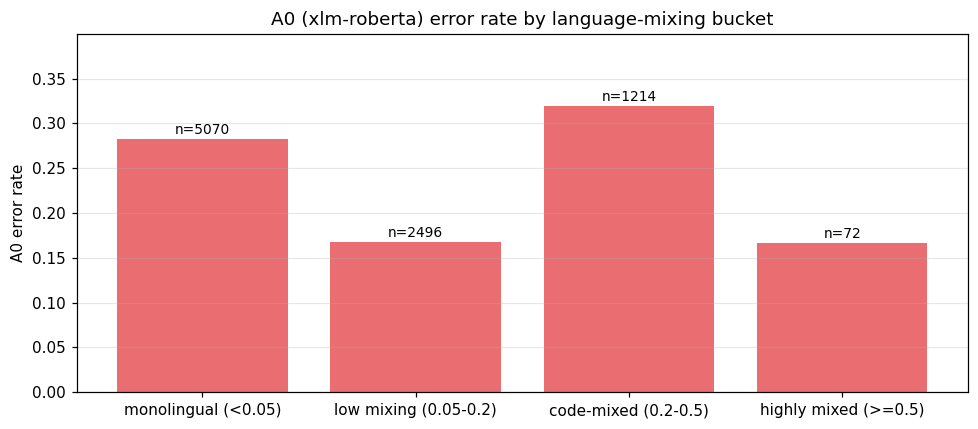
\includegraphics[width=0.62\textwidth]{figures/fig_error_phenomena.png}
\caption[A0 error rate by language-mixing bucket]{A0 (XLM-R) error rate by language-mixing bucket. The code-mixed bucket
is the peak of the error surface.}
\label{fig:errors}
\end{figure}

The reading is that \emph{true} code-switching---not romanisation alone, which
the subword vocabulary handles---remains the failure core of the task. A post
that alternates languages every few words (9.5 switches on average in the hard
bucket) requires the model to hold both languages' context in play, and neither
pretraining corpus taught it to do that at this frequency.

\subsection{Confusion structure}
Figure~\ref{fig:confusion} juxtaposes the two confusion matrices. The transformer
converts a large block of B0's non-hate errors into correct predictions (its
non-hate recall is 0.824 vs.\ 0.740) while its hate column looks similar to the
baseline's---consistent with \S\ref{sec:perclass}: the bought points are mostly
better \emph{non-hate} discrimination, i.e.\ fewer false accusations, while hate
recall barely moves (0.645 vs.\ 0.670).

\begin{figure}[htbp]
\centering
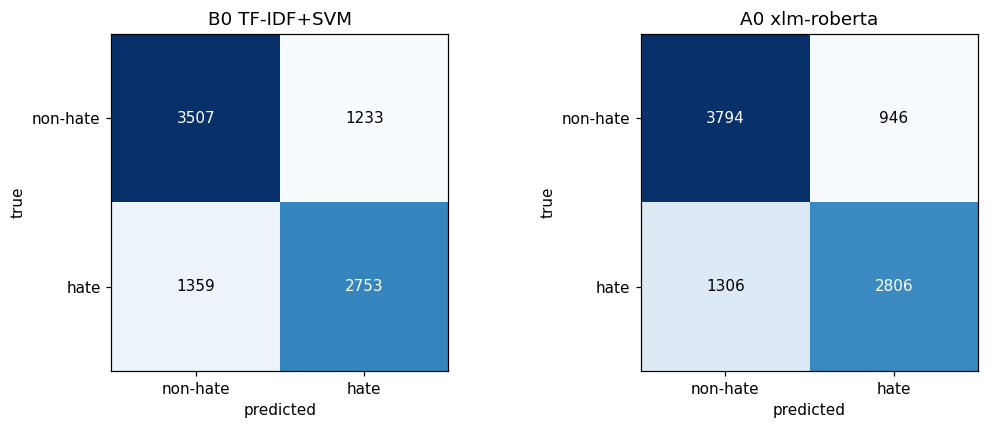
\includegraphics[width=0.72\textwidth]{figures/fig_confusion.png}
\caption[Confusion matrices: B0 vs.\ A0 (seed 42)]{Test-set confusion matrices (seed 42): B0 (left) vs.\ the
validation-selected A0 model (right).}
\label{fig:confusion}
\end{figure}

\subsection{Qualitative disagreements}
\label{sec:qualitative}
Table~\ref{tab:qualitative} shows posts on which B0 and A0 disagree, drawn from
the exported disagreement file (2{,}022 examples). The cases the transformer fixes
are long, sarcastic or implicit posts where lexical overlap misleads the linear
model; the cases it breaks are often short or borderline. Examples are shown in
Roman script; the export file also contains Devanagari rows.

\begin{table}[htbp]
\centering
\caption[Representative B0-vs-A0 disagreements]{Representative B0-vs-A0 disagreements (from 2{,}022 exported cases).
Posts are shown truncated; placeholders are the de-identification tokens of
\S\ref{sec:deid}.}
\label{tab:qualitative}
\scriptsize
\begin{tabular}{p{5.3cm}lccp{1.6cm}}
\toprule
Post (truncated) & True & B0 & A0 & Pattern \\
\midrule
``why are you making me jump through hoops when \ldots'' & 0 & 1 & 0 & A0 fixes false alarm \\
``laughing my ass off you guys i remember when s\ldots'' & 0 & 1 & 0 & A0 fixes false alarm \\
``are your friends safe living with a crush on y\ldots'' & 1 & 1 & 0 & A0 misses hate \\
``and you know he is probably saying the softest\ldots'' & 1 & 0 & 1 & A0 fixes miss \\
``give this up here is something you should take\ldots'' & 1 & 1 & 0 & A0 misses hate \\
\bottomrule
\end{tabular}
\end{table}

\section{Zero-Shot Cross-Lingual Transfer}
\label{sec:transfer}

Finally, the validation-selected model is applied, without any retraining, to the
416-post Marathi--English code-mixed test split of L3Cube-MeHate, carrying the
PRISM-validation threshold (0.53) unchanged. Table~\ref{tab:transfer} and
Figure~\ref{fig:transferfig} report the outcome: macro-F1 collapses from 0.7351
to 0.3770 (95\% CI $[0.3454, 0.4088]$)---a drop of 0.3581, and below the 0.5
level of a majority-vote classifier on this balanced set.

\begin{table}[htbp]
\centering
\caption[Zero-shot transfer from PRISM to MeHate]{Zero-shot transfer of the validation-selected A0 model (XLM-R, seed 42)
from PRISM (Hindi--English) to MeHate (Marathi--English), $n = 416$.}
\label{tab:transfer}
\small
\begin{tabular}{lrr}
\toprule
Setting & Macro-F1 & 95\% CI \\
\midrule
PRISM test (in-domain) & 0.7351 & [0.7265, 0.7439] \\
MeHate zero-shot (cross-lingual) & 0.3770 & [0.3454, 0.4088] \\
\midrule
Drop & 0.3581 & \\
\bottomrule
\end{tabular}
\end{table}

\begin{figure}[htbp]
\centering
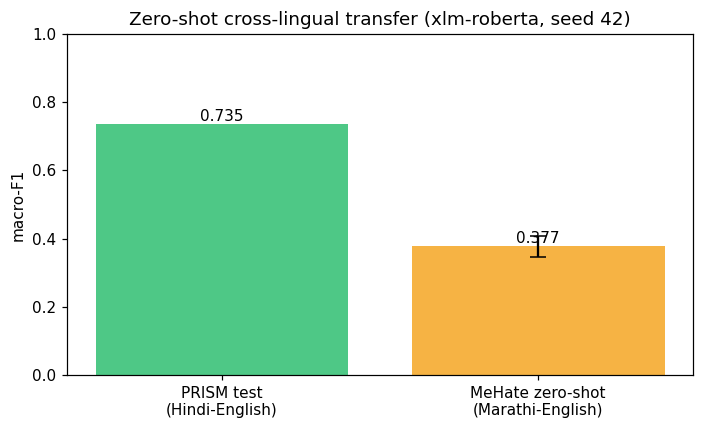
\includegraphics[width=0.48\textwidth]{figures/fig_transfer.png}
\caption[Zero-shot cross-lingual transfer]{Zero-shot cross-lingual transfer. The model that wins in-domain fails to
reach even chance-level behaviour out of domain.}
\label{fig:transferfig}
\end{figure}

Three confounds make the failure interpretable rather than merely embarrassing:
Marathi is (weakly) represented in XLM-R's pretraining but the fine-tuning
distribution is entirely Hindi--English; the MeHate split is small enough that
the CI is wide ($\pm$0.03); and the threshold was tuned for a different
probability calibration. Even granting all three, the conclusion stands: the
three-point in-domain advantage of pretraining does \emph{not} buy language
robustness for free. Transfer to a neighbouring Indian language fails, so the
idea of simply applying the PRISM model elsewhere is off the table, and
cross-lingual adaptation moves squarely into future work.

\section{Discussion}
\label{sec:discussion}

Returning to the problem statement: under an identical protocol, pretrained
multilingual encoders beat a character-level lexical baseline by about three
macro-F1 points on Hinglish hate-speech detection, the gain is significant under
Holm-corrected McNemar for every transformer, and the cost is roughly two orders
of magnitude in training time and one in inference latency.

The structure of the gain is as informative as its size. Pretraining bought
almost all of its improvement on English and lightly-mixed posts---the segments
where subword vocabulary robustness and world knowledge plausibly help---and
almost none on Devanagari Hindi or heavily code-switched posts, and none at all
out of domain. Domain-matched pretraining (HingRoBERTa) did not convert its
advantage into a win over the generalist, which suggests that at this data scale
the \emph{encoder capacity} matters more than the exact pretraining mixture, or
that 3 epochs of fine-tuning cannot re-align a domain-matched encoder better than
a strong general one. Both readings are consistent with the overlapping
confidence intervals and must be stated as hypotheses rather than findings.

The deployment-facing summary is threefold. First, the TF-IDF+SVM baseline is a
legitimate component, not a straw man: it costs seconds and reaches 0.7050. Any
report that compares transformers against nothing would overstate the value of
the GPU. Second, if the additional three points are needed, XLM-R is the
defensible choice, selected on validation, significant against the baseline. But
third---and this is the practical caveat---the added points concentrate on
non-hate recall, not on hate recall; the model that misses one hate post in three
gets only modestly less missed. For the actual goal of moderation, the hate
recall ceiling, not the leaderboard, is the frontier, and \S\ref{sec:future}
proposes the levers for it.

% =====================================================================
% CHAPTER 5 — CONCLUSIONS AND FUTURE WORK
% =====================================================================
\chapter{Conclusions and Future Work}
\label{ch:conclusion}

\section{Conclusions}
\label{sec:conclusions}

This study asked how much accuracy pretrained multilingual encoders buy over a
lexical baseline for binary hate-speech detection in Hinglish, under one shared
protocol and an explicitly leakage-safe evaluation. The five conclusions below
correspond to the five contributions of \S\ref{sec:contrib}.

\begin{enumerate}
\item \textbf{Pretraining wins by three points, significantly.} The TF-IDF +
linear-SVM baseline reaches 0.7050 test macro-F1; the transformers reach 0.7300
(HingRoBERTa), 0.7254 (MuRIL) and 0.7351 (XLM-R). All three gains are significant
against the baseline under exact McNemar with Holm correction, with $p$-values
between $10^{-4}$ and $10^{-13}$.
\item \textbf{The domain-matched encoder does not win.} HingRoBERTa, pretrained on
romanised Hinglish, finishes below the 100-language generalist XLM-R
(0.7300 vs.\ 0.7351) with heavily overlapping confidence intervals; MuRIL trails
both. At this data scale, three epochs of fine-tuning cannot be shown to exploit
domain-matched pretraining better than a strong generalist.
\item \textbf{The gain has a price and a shape.} The three F1 points cost roughly
$96\times$ the training time and $13\times$ the inference latency; they
concentrate on non-hate recall (0.824 vs.\ 0.740) while hate recall barely moves
(0.645 vs.\ 0.670), and they leave the code-mixed error peak (32.0\% error rate)
standing.
\item \textbf{Evaluation discipline changed the outcome.} Selecting the backbone
on validation rather than on test (the v1 defect) is not cosmetic: the protocol
now guarantees reported test numbers free of model-selection bias. The threshold
sweep, run on validation only, is worth at most $+0.0022$ F1 over the default
rule---a useful negative result that closes an unexamined degree of freedom.
\item \textbf{In-domain gains do not transfer.} The best model applied zero-shot
to Marathi--English collapses from 0.7351 to 0.3770 macro-F1---below a
majority-vote classifier. Cross-lingual robustness is not a free by-product of
Hinglish fine-tuning.
\end{enumerate}

\section{Limitations}
\label{sec:limits}

Table~\ref{tab:limits} collects the limitations of this study together with their
practical impact and the direction in which each can be addressed. They are
stated here rather than discovered by the reader.

\begin{table}[htbp]
\centering
\caption{Limitations, their impact, and improvement directions.}
\label{tab:limits}
\small
\begin{tabular}{>{\raggedright\arraybackslash}p{3.7cm}>{\raggedright\arraybackslash}p{5.2cm}>{\raggedright\arraybackslash}p{4.4cm}}
\toprule
Limitation & Impact & Direction \\
\midrule
Binary labels only & No target-group or severity analysis & Multiclass PRISM variants; hierarchical heads \\
Three seeds & Transformer std 0.004--0.006; transformer-vs-transformer gaps untestable & Five or more seeds; paired tests among A0 models \\
Lexicon-based mixing metric & Mixing index is a lower bound on true mixing & Model-based language ID (e.g.\ fastText per token) \\
MeHate transfer set: 416 posts, test split only & Wide CI ($\pm$0.03); no threshold re-tuning possible & Larger MeHate splits; small validation subset for calibration \\
Fixed 3-epoch, single-config budget & Under-tuned transformers; no LR ablation & Small sweep per backbone; report sensitivity \\
Hate recall ceiling untouched & Models miss $\sim$1 in 3 hate posts & Class-weighted loss, focal loss, hard-negative mining \\
Regex de-identification & Plain-text names survive & NER-based scrubbing before release \\
\bottomrule
\end{tabular}
\end{table}

\section{Future Work}
\label{sec:future}

Near term, three extensions follow directly from the error map. First, attack the
hate-recall ceiling: class-weighted or focal losses, and threshold tuning
optimising a recall floor instead of macro-F1, are one-line changes to the
existing harness and can be evaluated with the same three-seed protocol. Second,
make the mixing metric model-based (token-level language ID) so that the
code-mixed bucket can be analysed without lexicon bias. Third, run five seeds and
pairwise McNemar tests among the transformers so that the XLM-R vs.\ HingRoBERTa
question, deliberately left open here, gets an answer.

Medium term, the transfer failure deserves a dedicated study: adapter-based or
LoRA fine-tuning on a small Marathi--English validation sample, calibrated
thresholds per target domain, and a cascade architecture in which the cheap SVM
handles confident posts and the transformer only the ambiguous middle band
(\S\ref{sec:cost}). The disagreement export of \S\ref{sec:qualitative}---2{,}022
labelled cases---is a ready-made starting set for mining hard examples.

Long term, the pipeline is designed to generalise beyond one corpus: swapping the
loader in Section~1 for any binary hate-speech dataset with a \emph{text, label,
language} schema re-runs the whole study, and the pipeline's built-in self-tests
verify the new plumbing before any GPU minute is spent.


% =====================================================================
% REFERENCES
% =====================================================================
% =====================================================================
% REFERENCES
% =====================================================================
\begin{thebibliography}{11}
\addcontentsline{toc}{chapter}{References}
\sloppy

\bibitem{hingroberta}
L3Cube-Pune, ``HingRoBERTa: Hindi-English code-mixed RoBERTa,'' Hugging Face
model card. [Online]. Available: \url{https://huggingface.co/l3cube-pune/hing-roberta}


\bibitem{nayak2022}
R.~Nayak and R.~Joshi, ``L3Cube-HingCorpus and HingBERT: A code mixed
Hindi-English dataset and BERT language models,'' in \emph{Proc.\ WILDRE-6
Workshop @ LREC}, Marseille, France, 2022.


\bibitem{muril}
S.~Khanuja, D.~Bansal, S.~Mehtani, \emph{et~al.}, ``MuRIL: Multilingual
representations for Indian languages,'' \emph{arXiv preprint} arXiv:2103.10730,
2021.


\bibitem{xlmr}
A.~Conneau \emph{et~al.}, ``Unsupervised cross-lingual representation learning at
scale,'' in \emph{Proc.\ 58th Annual Meeting of the ACL}, 2020, pp.~8440--8451.


\bibitem{prism}
Pankajbiswas6, ``PRISM: Hinglish hate speech dataset
(\texttt{pankajbiswas6/prism-hinglish-hate-speech}),'' Hugging Face datasets,
revision \texttt{b27f83eb} (pinned in the pipeline). [Online]. Available:
\url{https://huggingface.co/datasets/pankajbiswas6/prism-hinglish-hate-speech}


\bibitem{mehate}
L3Cube-Pune, ``L3Cube-MeHate: Marathi hate speech detection dataset,''
\texttt{l3cube-pune/MarathiNLP}, commit \texttt{8ee29fa} (pinned). [Online].
Available: \url{https://github.com/l3cube-pune/MarathiNLP}


\bibitem{sklearn}
F.~Pedregosa \emph{et~al.}, ``Scikit-learn: Machine learning in Python,''
\emph{Journal of Machine Learning Research}, vol.~12, pp.~2825--2830, 2011.


\bibitem{bootstrap}
B.~Efron and R.~J.~Tibshirani, \emph{An Introduction to the Bootstrap}.
New York: Chapman \& Hall/CRC, 1993.


\bibitem{mcnemar}
Q.~McNemar, ``Note on the sampling error of the difference between correlated
proportions or percentages,'' \emph{Psychometrika}, vol.~12, no.~2,
pp.~153--157, 1947.


\bibitem{holm}
S.~Holm, ``A simple sequentially rejective multiple test procedure,''
\emph{Scandinavian Journal of Statistics}, vol.~6, no.~2, pp.~65--70, 1979.


\bibitem{transformers}
T.~Wolf \emph{et~al.}, ``Transformers: State-of-the-art natural language
processing,'' in \emph{Proc.\ EMNLP: System Demonstrations}, 2020, pp.~38--45.

\end{thebibliography}


% =====================================================================
% APPENDIX
% =====================================================================
% =====================================================================
% APPENDIX A — GLOSSARY OF TERMS
% =====================================================================
\appendix
\chapter{Glossary of Terms}
\label{app:glossary}
\begingroup\small\setstretch{1.0}

This appendix explains every technical term used in the report, in the order a
newcomer is likely to meet it: first the task and the language phenomenon, then
the models and their training, then the evaluation metrics---with their
formulas---and finally the statistical machinery that turns scores into claims.
Each entry is written to be self-contained; no entry assumes another.

\vspace{4pt}
\noindent\textbf{Code and demo availability.} The complete pipeline, the executed
notebook and all artifacts (result tables, figures, run manifest and
requirements freeze) are maintained in the project's GitHub repository with
regular commits from both team members. The working demo---the fully executed
Kaggle notebook, including every output and figure in this report---is available
at \url{https://www.kaggle.com/code/anishdate/code-mixed-hate-speech-detection-pipeline-v2}.

\section{Task and Language Terms}
\label{app:task}

\textbf{Hate speech detection.} The classification task, given a post, of deciding
whether it expresses hate or attacks a person or group (label 1, \emph{hate}) or
does not (label 0, \emph{non-hate}). This study uses the binary form; datasets
that distinguish target groups or severity are outside its scope.

\textbf{Code-mixed language.} Text in which two or more languages alternate
within the same sentence or phrase, without typographic separation---from a single
borrowed word to a full clause switch; the ``mixing index'' entry below gives the
measure used here.

\textbf{Hinglish.} The Hindi--English code-mixed register dominant on Indian
social media: Hindi written in the Roman script (``romanised Hindi''), freely
interspersed with English words. Written Hindi normally uses the Devanagari
script; the Roman-script form has no standard spelling.

\textbf{Romanisation.} Writing a non-Latin script with Latin letters. Because it
is done by ear, one Hindi word acquires many spellings (\emph{hai}, \emph{hain},
\emph{he}, \emph{hn})---the main reason word-level vocabularies fragment and
character-level or subword models cope better.

\textbf{De-identification.} Removing personal information from text before
analysis: here, replacing URLs, email addresses, phone numbers and @handles with
placeholders, and collapsing letter elongation. Regex-based de-identification does
not catch plain-text names (Table~\ref{tab:limits}).

\textbf{PII.} Personally identifiable information: names, handles, phone numbers,
addresses and similar data that can identify a person.

\textbf{Data card.} A metadata file written next to a processed dataset,
recording its source, revision, licence, split sizes and preprocessing rules, so
that the data behind an experiment is auditable.

\textbf{Class imbalance.} A mismatch between the number of examples of each
class. PRISM is mildly imbalanced (53.5\% / 46.5\%), which is why macro-averaged
metrics are preferred over raw accuracy.

\section{Models and Training Terms}
\label{app:models}

\textbf{TF-IDF.} Term frequency--inverse document frequency. A way of turning text
into numbers: each feature counts how often a term occurs in a post (TF), down-weighted
by how common the term is across all posts (IDF), so that ubiquitous words carry
little signal.

\textbf{Character $n$-gram.} A substring of $n$ consecutive characters
(\emph{hain} contains the 3-grams \emph{hai} and \emph{ain}). Char $n$-grams
match misspelled and romanised variants through shared substrings and need no
dictionary---the reason the B0 baseline uses them with $n$ from 2 to 5.

\textbf{Linear SVM.} A linear support vector machine: it learns a weighted
combination of features and classifies by the sign of the score. It has no
probability output (hence no threshold to tune) and trains in seconds.

\textbf{Baseline.} A deliberately simple reference model that defines the score a
new method must beat. B0 (TF-IDF + SVM) plays this role: without it, a
transformer's three-point gain would have no costed reference point.

\textbf{Transformer.} The neural architecture underlying modern NLP: all tokens
are processed in parallel through stacked blocks of self-attention and
feed-forward layers, trained by gradient descent.

\textbf{Self-attention.} The mechanism by which every token computes a weighted
view of every other token, letting the model connect, say, a pronoun with the
noun it refers to several words away.

\textbf{Pretrained language model.} A transformer that has already been trained on
a large unlabelled corpus and therefore knows spelling, syntax and some world
knowledge before the task-specific training starts. HingRoBERTa, MuRIL and XLM-R
are three such models with different pretraining corpora.

\textbf{Fine-tuning.} Continuing to train a pretrained model on a small labelled
dataset (here: 17{,}704 posts, 3 epochs) so that its general language knowledge is
re-pointed at the task. All transformer results here are fine-tuned models.

\textbf{Classification head.} The small layer added on top of a pretrained
encoder that maps its output to the two class scores. It starts from random
weights and is trained together with (or on top of) the encoder.

\textbf{Epoch, batch, learning rate.} One \emph{epoch} is a pass over the
training data; training proceeds in \emph{batches} of 32 posts; the \emph{learning
rate} ($2\times10^{-5}$) is the optimiser's step size.

\textbf{Warmup and weight decay.} \emph{Warmup} (ratio 0.1) raises the learning
rate gradually over the first 10\% of steps, avoiding instability at the start;
\emph{weight decay} (0.01) penalises large weights, a mild regulariser.

\textbf{fp16 (mixed precision).} Storing and multiplying most network values in
16-bit instead of 32-bit floats, roughly halving GPU memory and speeding up
training. Small numerical differences remain, which is why seeds are described as
``reproducible in practice'' rather than bit-exact.

\textbf{Seed.} The number that starts all pseudo-random processes (weight
initialisation, shuffling, dropout). Re-running with seeds 42, 43, 44 measures
how much of the score is luck.

\textbf{Checkpoint.} A snapshot of the model saved during training. The pipeline
saves one per epoch and restores the one with the best \emph{validation} macro-F1,
not the final one.

\section{Evaluation Metrics}
\label{app:metrics}

All metrics are computed on a \textbf{confusion matrix}, the $2\times2$ table of
predicted vs.\ true classes. For the hate class: TP = hate posts predicted hate,
FP = non-hate posts predicted hate (false alarms), FN = hate posts predicted
non-hate (misses), TN = non-hate posts predicted non-hate.

\textbf{Precision} (per class) answers: ``of the posts the model called hate, how
many really were?''
\begin{equation}
\mathrm{Precision}_{c} = \frac{TP_{c}}{TP_{c} + FP_{c}}
\end{equation}

\textbf{Recall} (per class) answers: ``of the posts that really were hate, how
many did the model catch?''
\begin{equation}
\mathrm{Recall}_{c} = \frac{TP_{c}}{TP_{c} + FN_{c}}
\end{equation}

\textbf{F1} (per class) is the harmonic mean of the two---a class scores well on
F1 only if both precision and recall are high:
\begin{equation}
F_{1,c} = \frac{2\,\mathrm{Precision}_{c}\cdot\mathrm{Recall}_{c}}
               {\mathrm{Precision}_{c} + \mathrm{Recall}_{c}}
\end{equation}

\textbf{Macro-F1}---the primary metric of this report---is the unweighted average
of the per-class F1 over the $C$ classes ($C=2$ here):
\begin{equation}
\mFmac = \frac{1}{C}\sum_{c=1}^{C} F_{1,c}
\end{equation}
``Macro'' means each class counts equally. A model that is excellent on the large
class and useless on the small one gets a low macro-F1, which is exactly the
sensitivity wanted for hate speech: missing the hate class must cost as much as
failing on non-hate. This is why a 99\% accuracy on 99\% non-hate data would be
worthless, while macro-F1 would expose it as near zero.

\textbf{Macro precision / macro recall} apply the same unweighted averaging to
precision and recall. They are reported so that a macro-F1 change can be traced
to fewer false alarms (precision up) or fewer misses (recall up).

\textbf{MCC --- Matthews correlation coefficient.} A single-number summary of the
whole confusion matrix that is robust to imbalance, ranging from $-1$ (always
wrong) through 0 (random) to $+1$ (perfect):
\begin{equation}
\mathrm{MCC} =
\frac{TP\cdot TN - FP\cdot FN}
     {\sqrt{(TP+FP)(TP+FN)(TN+FP)(TN+FN)}}
\end{equation}

\textbf{Balanced accuracy} is the average of the two class recalls:
\begin{equation}
\mathrm{Balanced\ accuracy} = \tfrac{1}{2}\left(\frac{TP}{TP+FN} + \frac{TN}{TN+FP}\right)
\end{equation}
It ignores precision entirely, so comparing it with macro-F1 shows how much of a
model's quality comes from precision (fewer false alarms).

\textbf{Support.} The number of true examples of a class in the evaluated set.
Per-class scores are read against their support: the highly-mixed bucket of
Table~\ref{tab:buckets} carries only 72 posts, which is why its numbers move
widely.

\textbf{Decision threshold.} Transformers output a probability $p$ that a post is
hate; the \emph{threshold} $t$ turns it into a decision (hate if $p \geq t$).
The default $t = 0.5$ is a convention, not an optimum; this study tunes $t$ on
the validation set (\S\ref{sec:protocol}).

\clearpage
\section{Statistical and Protocol Terms}
\label{app:stats}

\textbf{Bootstrap confidence interval (CI).} A measure of how much a reported
number would wobble if the test set were redrawn. The test set is resampled with
replacement 1{,}000 times, the metric recomputed on each resample, and the 2.5th
and 97.5th percentiles form the 95\% CI. Within each resample the three seeds are
averaged, so the interval surrounds the plotted 3-seed mean.

\textbf{Seed variance / standard deviation.} The spread of a metric across seeds
42, 43, 44. It measures training luck, not test-set luck; both must be small
before two models can be ranked.

\textbf{McNemar's test.} A significance test for two models on the same items;
only the \emph{discordant} pairs matter---items where exactly one model is
correct. Under the null hypothesis ``both are equally good'', the split
$n_{10}$ vs.\ $n_{01}$ is a fair coin toss, and the exact binomial test on
$\min(n_{01}, n_{10})$ out of $n_{01}+n_{10}$ gives the $p$-value. It is the
correct paired test here because both models label the identical 8{,}852 posts.

\textbf{$p$-value.} The probability, assuming two models are in fact equally
good, of seeing a discrepancy at least as large as the observed one. A small
$p$-value is evidence \emph{against} equality, not a proof of importance.

\textbf{Holm correction.} When several hypotheses are tested at once (here: three
transformers each vs.\ the baseline), the chance of a false ``significant'' grows.
The Holm procedure orders the $p$-values and multiplies the $i$-th smallest by
$(m - i + 1)$, capping at 1, which keeps the family-wise error rate at the nominal
level. All ``significant'' claims in this report use Holm-adjusted $p$-values.

\textbf{Zero-shot transfer.} Applying a model to a domain or language it was never
trained on---here, the PRISM-trained model applied to Marathi--English posts with
no retraining and the same threshold. The 0.3770 result shows the term is not a
formality: zero-shot can fail completely.

\textbf{Data leakage.} Any route by which information from the test set influences
training or model selection, inflating reported scores. The v1$\rightarrow$v2 fix
(\S\ref{sec:protocol}) removed one concrete route: selecting the backbone on test
macro-F1.

\textbf{Validation set / test set.} The validation set (2{,}950 posts) is the
``exam for feedback'': all tuning and selection decisions read it. The test set
(8{,}852 posts) is the ``final exam'', touched once per seed for reporting.
Keeping the channels separate is what makes the reported numbers mean what they
claim.
\endgroup


\end{document}
